\section{Tensor Networks Basics}\label{chapter:basics}

As their order increases, representing and working with tensors becomes more complicated. 
Tensor networks provide an efficient framework for working with these high-order objects, simplifying both their representation and analysis. 
The graphical notation of tensor networks offers an intuitive way to visualize and simplify complex tensor operations~\citep{orus2014practical,biamonte2017tensor}. 
In this section, we introduce basic notions on tensors and common tensor operations using the language of tensor networks.

\subsection{What are Tensor Networks?}
As their name suggests, Tensor Networks (TNs) are simply tensors connected to each other to form a network. More precisely, a tensor network is a graph in which vertices represent \emph{tensors} and edges represent \emph{contracted} indices (shared modes). The graphical notation for tensor networks was first introduced by~\cite{penrose1971applications}. Tensors are represented by shapes with legs~(edges), i.e.,
$
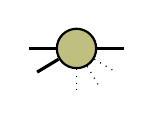
\begin{tikzpicture}[baseline=-0.5ex]
    \tikzset{tensor/.style = {minimum size = 0.5cm,shape = circle,thick,draw=black,inner sep = 0pt}, edge/.style = {thick,line width=.4mm},every loop/.style={}}
    \def\x{6}
    \node[tensor,fill=green!50!red!50!white] (T) at (\x,0) {$\Tt$};
    \draw[edge] (T) -- (\x-0.6,0);
    \draw[edge] (T) -- (\x+0.6,0);
    \draw[edge] (T) -- (\x-0.5,-0.3);
    \draw[dotted] (T) -- (\x,-0.6);
    \draw[dotted] (T) -- (\x+0.5,-0.3);
    \draw[dotted] (T) -- (\x+0.3,-0.5);
    \end{tikzpicture}.
$
We will use different shapes, such as rectangles, triangles, or circles, and various colors to represent tensors. Shapes and colors serve mainly as visual cues. 
The \emph{order} of a tensor is its number of dimensions, e.g., an $N$-th order tensor $\Tt\in\RR^{d_1\times\cdots\times d_N}$ is a multidimensional array of scalars~$\Tt_{i_1,\dots,i_N}$ indexed by $N$ indices $i_1\in [d_1], i_2\in[d_2],\cdots, i_N \in [d_N]$. Each axis is called a \emph{mode} of a tensor: an $N$-th order tensor has $N$ modes.
 
 Tensors naturally generalize vectors and matrices to higher-order arrays. As the order increases, representing these arrays becomes more challenging. \emph{Tensor networks} provide a simple and intuitive way to represent and manipulate these higher-order objects. Complex operations on tensors can be represented more easily with graphical notations of tensor networks~\citep{biamonte2017tensor,orus2014practical}. 


\paragraph{Tensor Network Nodes}\label{def:tn-nodes}
In a tensor network, each node~(or vertex) represents a tensor, and the number of legs~(incident edges) corresponds to the order of the tensor: scalars are nodes with no edges, vector nodes have a single edge, matrix nodes have two edges, and so on. For example,
\begin{center}
    
    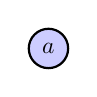
\begin{tikzpicture}[baseline=-0.5ex]
    \tikzset{tensor/.style = {minimum size = 0.5cm,shape = circle,thick,draw=black,inner sep = 0pt}, edge/.style = {thick,line width=.4mm},every loop/.style={}}
    \def\y{0}
    \def\x{0}
    \node[tensor,fill=blue!20!white] (a) at (\x,\y){\scalebox{0.85}{$a$}};
    \end{tikzpicture}%
    \ \ \ $\in \RR$,\hspace{0.01cm}
    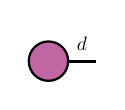
\begin{tikzpicture}[baseline=-0.5ex]
    \tikzset{tensor/.style = {minimum size = 0.5cm,shape = circle,thick,draw=black,inner sep = 0pt}, edge/.style = {thick,line width=.4mm},every loop/.style={}}
    \def\y{0}
    \def\x{0}
    \node[tensor,fill=blue!40!red!60!white] (a) at (\x,\y){\scalebox{0.85}{$\ab$}};
    \draw[edge] (\x+0.25,\y) -- (\x+0.6,\y)  node [midway,above] {\scalebox{0.7}{\dimcolor{$d$}}};
    \end{tikzpicture}
    $\in \RR^d$,\hspace{0.3cm}
    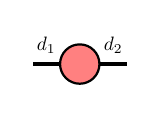
\begin{tikzpicture}[baseline=-0.5ex]
    \tikzset{tensor/.style = {minimum size = 0.5cm,shape = circle,thick,draw=black,inner sep = 0pt}, edge/.style = {thick,line width=.4mm},every loop/.style={}}
    \def\y{0}
    \def\x{0}
    \node[tensor,fill=red!50!white] (A) at (\x,\y){\scalebox{0.85}{$\Ab$}};
    \draw[edge] (\x+0.25,\y) -- (\x+0.6,\y)  node [midway,above] {\scalebox{0.7}{\dimcolor{$d_2$}}};
    \draw[edge] (\x-0.25,\y) -- (\x-0.6,\y)  node [midway,above] {\scalebox{0.7}{\dimcolor{$d_1$}}};
    \end{tikzpicture}
    \ \ \ $\in \RR^{d_1\times d_2}$,\hspace{0.3cm}
    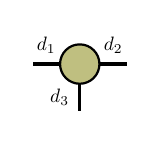
\begin{tikzpicture}[baseline=-0.5ex]
    \tikzset{tensor/.style = {minimum size = 0.5cm,shape = circle,thick,draw=black,inner sep = 0pt}, edge/.style = {thick,line width=.4mm},every loop/.style={}}
    \def\y{0}
    \def\x{0}
    \node[tensor,fill=green!50!red!50!white] (A) at (\x,\y){\scalebox{0.85}{$\At$}};
    \draw[edge] (\x+0.25,\y) -- (\x+0.6,\y)  node [midway,above] {\scalebox{0.7}{\dimcolor{$d_2$}}};
    \draw[edge] (\x-0.25,\y) -- (\x-0.6,\y)  node [midway,above] {\scalebox{0.7}{\dimcolor{$d_1$}}};
    \draw[edge] (\x,\y-0.25) -- (\x,\y-0.6)  node [midway,left] {\scalebox{0.7}{\dimcolor{$d_3$}}};
    \end{tikzpicture}
    \ \ \ $\in \RR^{d_1\times d_2\times d_3}$,\hspace{0.01cm}
    \begin{tikzpicture}[baseline=-0.5ex]
    \tikzset{tensor/.style = {minimum width = 1.8cm,minimum height = 0.4cm,shape = rounded rectangle,thick,draw=black,inner sep = 0pt}, edge/.style = {thick,line width=.4mm},every loop/.style={}}
    \def\x{0}
    \def\y{0}
    \draw[edge] (\x-0.2,\y-0.15) -- (\x-0.2,\y-0.6)node [midway,left=-0.05cm] {\scalebox{0.7}{\dimcolor{$d_2$}}};
    \draw[edge] (\x-0.6,\y-0.15) -- (\x-0.6,\y-0.6)node [midway,left=-0.05cm] {\scalebox{0.7}{\dimcolor{$d_1$}}};
    \draw[edge] (\x+0.2,\y-0.15) -- (\x+0.2,\y-0.6)node [midway,left=-0.05cm] {\scalebox{0.7}{\dimcolor{$d_3$}}};
    \draw[edge] (\x+0.6,\y-0.15) -- (\x+0.6,\y-0.6)node [midway,left=-0.05cm] {\scalebox{0.7}{\dimcolor{$d_4$}}};
    \node[tensor,fill=green!30!white] (Bt) at (\x,\y){$\Bt$};
    \end{tikzpicture}
    $\in \RR^{d_1\times d_2\times d_3\times d_4}$.

\end{center}
represent a scalar, a vector, a matrix, a third- and a fourth-order tensors, respectively. 
Throughout this manuscript,
\begin{itemize}
    \item Tensors are represented by colored shapes called nodes, where the colors and shapes have no specific meaning~(unless stated otherwise). 
    \item We use lower case letters for scalars~(e.g., $a$), bold lower case letters for vectors~(e.g., $\vb$), bold upper case letters for matrices (e.g., $\Mb$), and 
    bold upper case calligraphic letters for higher-order tensors~(e.g., $\Tt$).
    \item The dimension of each mode of a tensor is depicted by a gray letter positioned at the top of the corresponding leg, e.g., 
$
    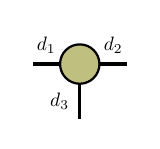
\begin{tikzpicture}[baseline=-0.5ex]
    \tikzset{tensor/.style = {minimum size = 0.5cm,shape = circle,thick,draw=black,inner sep = 0pt}, edge/.style = {thick,line width=.4mm},every loop/.style={}}
    \def\y{0}
    \def\x{0}
    \node[tensor,fill=green!50!red!50!white] (A) at (\x,\y){\scalebox{0.85}{$\At$}};
    \draw[edge] (\x+0.25,\y) -- (\x+0.6,\y)  node [midway,above] {\scalebox{0.7}{\dimcolor{$d_2$}}};
    \draw[edge] (\x-0.25,\y) -- (\x-0.6,\y)  node [midway,above] {\scalebox{0.7}{\dimcolor{$d_1$}}};
    \draw[edge] (\x,\y-0.25) -- (\x,\y-0.7)  node [midway,left] {\scalebox{0.7}{\dimcolor{$d_3$}}};
    \end{tikzpicture}
    \ \ \ \in \RR^{d_1\times d_2\times d_3},
$
is a third-order tensor of size $d_1\times d_2\times d_3$.
    
$
\At_{i,j,k} = 
    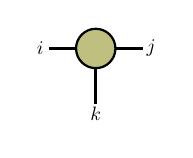
\begin{tikzpicture}[baseline=-0.5ex]
    \tikzset{tensor/.style = {minimum size = 0.5cm,shape = circle,thick,draw=black,inner sep = 0pt}, edge/.style = {thick,line width=.4mm},every loop/.style={}}
    \def\y{0}
    \def\x{0}
    \node[tensor,fill=green!50!red!50!white] (A) at (\x,\y){\scalebox{0.85}{$\At$}};
    \draw[edge] (\x+0.25,\y) -- (\x+0.6,\y)  node [pos=1.3] {\scalebox{0.7}{\indcolor{$j$}}};
    \draw[edge] (\x-0.25,\y) -- (\x-0.6,\y)  node [pos=1.3] {\scalebox{0.7}{\indcolor{$i$}}};
    \draw[edge] (\x,\y-0.25) -- (\x,\y-0.7)  node [pos=1.3] {\scalebox{0.7}{\indcolor{$k$}}};
    \end{tikzpicture}
$    
is the $(i,j,k)$-th element of the third-order tensor $\At$.
\end{itemize}
Note that large matrices can sometimes be viewed as high-order tensors through reshaping, e.g., 
\begin{align*}
    &\Tb
    =
    \begin{tikzpicture}[baseline=\baseline]
    \tikzset{tensor/.style = {minimum size = 0.5cm,shape = circle,thick,draw=black,inner sep = 0pt}, edge/.style = {thick,line width=.4mm},every loop/.style={}}
    \def\x{0}
    \def\y{0}
    \node[tensor,fill=green!50!blue!40!white] (Tb) at (\x,\y){$\Tb$};
    \draw[edge] (Tb) -- (\x+1.15,\y) node [midway,above] {\scalebox{0.7}{\dimcolor{$J_1J_2J_3J_4$}}};
    \draw[edge] (Tb) -- (\x-1.15,\y) node [midway,above] {\scalebox{0.7}{\dimcolor{$I_1I_2I_3I_4$}}};
    \end{tikzpicture}\in\RR^{I_1I_2I_3I_4\times J_1J_2J_3J_4}
    \equiv
    \Tt = 
    \begin{tikzpicture}[baseline=-0.5ex]
    \tikzset{tensor/.style = {minimum width = 1.8cm,minimum height = 0.4cm,shape = rounded rectangle,thick,draw=black,inner sep = 0pt}, edge/.style = {thick,line width=.4mm},every loop/.style={}}
    \def\x{0}
    \def\y{0}
    \draw[edge] (\x-0.2,\y-0.15) -- (\x-0.2,\y-0.6)node [midway,left=-0.05cm] {\scalebox{0.7}{\dimcolor{$I_2$}}};
    \draw[edge] (\x-0.6,\y-0.15) -- (\x-0.6,\y-0.6)node [midway,left=-0.05cm] {\scalebox{0.7}{\dimcolor{$I_1$}}};
    \draw[edge] (\x+0.2,\y-0.15) -- (\x+0.2,\y-0.6)node [midway,left=-0.05cm] {\scalebox{0.7}{\dimcolor{$I_3$}}};
    \draw[edge] (\x+0.6,\y-0.15) -- (\x+0.6,\y-0.6)node [midway,left=-0.05cm] {\scalebox{0.7}{\dimcolor{$I_4$}}};
    \draw[edge] (\x-0.2,\y+0.15) -- (\x-0.2,\y+0.6)node [midway,left=-0.05cm] {\scalebox{0.7}{\dimcolor{$J_2$}}};
    \draw[edge] (\x-0.6,\y+0.15) -- (\x-0.6,\y+0.6)node [midway,left=-0.05cm] {\scalebox{0.7}{\dimcolor{$J_1$}}};
    \draw[edge] (\x+0.2,\y+0.15) -- (\x+0.2,\y+0.6)node [midway,left=-0.05cm] {\scalebox{0.7}{\dimcolor{$J_3$}}};
    \draw[edge] (\x+0.6,\y+0.15) -- (\x+0.6,\y+0.6)node [midway,left=-0.05cm] {\scalebox{0.7}{\dimcolor{$J_4$}}};
    \node[tensor,fill=yellow] (Bt) at (\x,\y){$\Tt$};
    \end{tikzpicture}
    \in\RR^{I_1\times I_2\times I_3\times I_4\times J_1 \times J_2\times J_3\times J_4}.
\end{align*}
\paragraph{Tensor Network Edges}\label{subsec:contraction} In tensor network diagram, legs are of two types: contracted legs~(those connecting two tensors) and un-contracted legs, also called free legs, with one dangling end~(i.e., a leg that is not connected to any other tensor). As mentioned above, un-contracted legs correspond to free indices:  the number of free legs indicates the order of a tensor: scalars have no free legs, vectors have one, matrices have two, and higher-order tensors have three or more.  Contracted legs represent contractions: 
tensors can be connected along legs of the same size, which represents a summation~(contraction) over the connected modes. 
We use the terms summation and contraction interchangeably. The most common contraction operation is \textit{matrix multiplication}. For two matrices $\Ab\in\RR^{d_1\times R}, \Bb\in\RR^{R\times d_2}$, their matrix product corresponds to a contraction between the second mode of $\Ab$ and the first mode of $\Bb$:

\begin{align}\label{eq:matrix-product}
(\Ab\Bb)_{ij} 
=
\begin{tikzpicture}[baseline=\baseline]
   \tikzset{tensor/.style = {minimum size = 0.5cm,shape = circle,thick,draw=black,inner sep = 0pt}, edge/.style = {thick,line width=.4mm},every loop/.style={}}
    \def\y{0}
    \def\x{0}
    \node[tensor,fill=red!50!white] (A) at (\x,\y){\scalebox{0.85}{$\Ab$}};
    \node[tensor,fill=blue!50!white] (B) at (\x+1,\y){\scalebox{0.85}{$\Bb$}};
    \draw[edge] (A) -- (B) node [above,midway] {\scalebox{0.7}{\dimcolor{$R$}}};
    \draw[edge] (\x-0.25,\y) -- (\x-0.75,\y)  node [pos=1.3] {\scalebox{0.7} {\indcolor{$i$}}};
    \draw[edge] (\x+1.25,\y) -- (\x+1.75,\y)  node [pos=1.3] {\scalebox{0.7}{\indcolor{$j$}}};
    \end{tikzpicture}
= \sum_{r=1}^R\Ab_{ir}\Bb_{rj},\ \ \ \text{for}\ \ i\in[d_1],j\in[d_2]\ .
\end{align}
Since this equality is true for all indices $i$ and $j$, we can simply write
\begin{align}\label{eq:matrix-product_noidx}
\Ab\Bb 
=
\begin{tikzpicture}[baseline=\baseline]
   \tikzset{tensor/.style = {minimum size = 0.5cm,shape = circle,thick,draw=black,inner sep = 0pt}, edge/.style = {thick,line width=.4mm},every loop/.style={}}
    \def\y{0}
    \def\x{0}
    \node[tensor,fill=red!50!white] (A) at (\x,\y){\scalebox{0.85}{$\Ab$}};
    \node[tensor,fill=blue!50!white] (B) at (\x+1,\y){\scalebox{0.85}{$\Bb$}};
    \draw[edge] (A) -- (B) node [above,midway] {\scalebox{0.7}{\dimcolor{$R$}}};
    \draw[edge] (\x-0.25,\y) -- (\x-0.75,\y)  node [midway, above] {\scalebox{0.7}{\dimcolor{$d_1$}}};
    \draw[edge] (\x+1.25,\y) -- (\x+1.75,\y)  node [midway,above] {\scalebox{0.7}{\dimcolor{$d_2$}}};
    \end{tikzpicture}
 \ \in \mathbb R^{d_1\times d_2}.
\end{align}

